
%%
% bayesian data analyses

% guessing parameter only used in language tasks, not in prior elicitation
% expt1a
%	- prevalence for categories (e..g "lions" that "have manes"):  
%         -  Beta(gamma, delta)  --- gamma (uniform 0 1); delta  (uniform 0 50)
% 		- using posterior on gamma for model
%   - prevalence prior for properties (e.g. "have manes"): 
%		- theta_across (uniform 0 1)	
%         -  Beta(gamma_within, delta_within)  --- gamma (uniform 0 1); delta  (uniform 0 50)
% 		-  using posterior on beta for model
% expt1b
%   - speaker optimality
%	- phi
% expt 2a
%  - Beta_across (gamma_across, delta_across) - 
%  - Beta_within (gamma_within, delta_within) -
%  - phi
% expt 2b
%   - speaker optimality (truth conditions)
%   - speaker optimality (implied prevalence)
%	- 2 phis (1 per task)





% mh 7/19
% in experiment 1 and model, take the speaker perspective when talking about how the model works

%todo after cogsci:
%-run additional contexts. e.g. separate dangerous and distinct.
%-look again at finer-grained truth judgement task?
%-think about the weird cases of generics in the literature. e.g. ``robins lay eggs''.
% - try an S2 model of prevalence judgement task, too. does it reduce to the L1 model?

% comments from workshop class 4/29
%
% why spend a lot of time in replication?
% 7 --- summary sentence 2nd paragraph to intro
% abstract worrisome
% look at study discussions -- move stuff to intro
%
% Lay eggs vs. Are female /// John is tall vs. ESB is tall [move even earlier]
% Move "a natural foil" earlier
%
% Maybe add talk of stereotypes?
% Craig: Use speaker / listener actors more; think about the person and the thing they're doing
% %
%  beef up penultimate paragraph in intro: talk about why distinctive and dangerous are important
% ---- unpack distinctive and dangerous (use experimental materials)
%
% TABLE for materials and experiment. 
% maybe set up replication-idea early.  and then go on.




% details
%
% Section 4: exp 2 intro
%% oceans underneath each sentence
%% connect back with behavior--- asymmetry, truth cond
%
% pre Exp 3: use 
% "endemic to the entire category"
% exp3a: jargon word 
% (reuse penultimate intro paragraph throughout) [maybe make higher level version of this paragraph for intro]
%
% pre-experiments, "Like Exp 2c, 3b did BLAH but differed "
%
% add more to figure captions?
%
%
% seeds of very last paragraph in earlier
%
% in conclusion: what do the tools allow us to do? (e.g. w/ stereotyping) 
% differences in prior knowledge --> how does this contribute to language change?
% 

\documentclass[10pt,letterpaper]{article}

\usepackage{setspace}
%\doublespacing
\usepackage{geometry}
\geometry{legalpaper, margin=1in}

\usepackage{pslatex}
\usepackage{apacite}
\usepackage{url}
\usepackage{graphicx}
\usepackage{caption}
\usepackage{subcaption}
\usepackage{listings}
\usepackage{color}
\usepackage{textcomp}
\usepackage{amsmath}
\usepackage{amssymb}
\usepackage{wrapfig}
\usepackage{lipsum}


\graphicspath{{figures/}}

\def\signed #1{{\leavevmode\unskip\nobreak\hfil\penalty50\hskip2em
  \hbox{}\nobreak\hfil(#1)%
  \parfillskip=0pt \finalhyphendemerits=0 \endgraf}}

\newsavebox\mybox
\newenvironment{aquote}[1]
  {\savebox\mybox{#1}\begin{quote}}
  {\signed{\usebox\mybox}\end{quote}}


 \newcommand{\denote}[1]{\mbox{ $[\![ #1 ]\!]$}}

\definecolor{Red}{RGB}{255,0,0}
\newcommand{\red}[1]{\textcolor{Red}{#1}}  
\definecolor{Green}{RGB}{10,200,100}
\definecolor{Blue}{RGB}{10,100,200}
\newcommand{\ndg}[1]{\textcolor{Green}{[ndg: #1]}}  
\newcommand{\mht}[1]{\textcolor{Blue}{[mht: #1]}}  

\usepackage{titlesec}

\setcounter{secnumdepth}{4}

\titleformat{\paragraph}
{\normalfont\normalsize\bfseries}{\theparagraph}{1em}{}
\titlespacing*{\paragraph}
{0pt}{3.25ex plus 1ex minus .2ex}{1.5ex plus .2ex}

\title{Generics are vague: A formal account of generalizations in language}
%\title{Generics are vague: a probabilistic model of generic language}
%\title{Generic language is vague yet rationally understood}
%\title{Generic language is vague yet pragmatically understood}
%\title{Generic language is vague yet pragmatically used}

\author{{\large \bf Michael Henry Tessler} (mtessler@stanford.edu)\\ {\large \bf Noah D. Goodman} (ngoodman@stanford.edu) \\
  Department of Psychology, Stanford University}
 
\begin{document}

\maketitle

%\mht{Notes: In this draft, I tried using different terminology for prevalence in the manuscript, which become more specific as you move into the manuscript. I start describing it as ``evidence'', a la the evidence a speaker needs to justify the sentence. I then use the term ``statistics'' to contrast the view with the rule-based / mental repertoire account of Leslie. Finally, I use the term prevalence only when introducing the model.}

\begin{abstract}

%\mht{revised: word-length realistic (limit 150)}
%\ndg{i don't like this abstract.}
%
%Generalizations about categories (e.g.~\emph{Dogs bark.}) are ubiquitous in everyday conversation. 
%Despite their prevalence, these \emph{generic} statements are puzzling to formal theories and their precise meanings are unknown. 
%Generics can in some instances be felicitous based on a small amount of evidence while other times require strong evidence to be true. 
%Generics are also difficult to understand formally because they tend to exaggerate how widespread the property (e.g. ``barks'') is within the category (e.g. ``dogs'').
%% tends to exaggerate how widespread the property being discussed \mht{better word?}  is.
%%the most common way to express generalizations about categories.
%%Generic utterances (e.g. ``Dogs bark.'') are the primary vessel by which speakers express ideas about categories in the world and are ubiquitous in everyday conversation. 
%%It is believed that generic utterances behave somewhat like quantified ones (e.g. ``Most dogs bark.''). 
%%If this is correct, however, there should be some threshold on the number of instances that display the property (e.g. some criterion number of dogs that bark) for the utterance to be true.
%%This threshold is notoriously difficult to define for generics, which are flexible enough to be true based on very little evidence while also implying near-universality of the property. 
%We explore the idea that the meaning of generic language is vague or uncertain and demonstrate how a theory of pragmatic language understanding can 
%%introduce a semantics and pragmatics for generic language understanding, centered on the idea that generics are vague. 
%%The criterion for truth is represented as an unknown property of the language and is actively reasoned about in context by a listener who assumes she is in conversation with an informative speaker. 
%%We explain how this simple semantics can
%operate over this under-specific meaning to explain these two outstanding puzzles. 
%%the variable implications of generic language. 
%%Inferences from the model are driven largely by the hypothetical interpreter's beliefs about the property.
%The model of language interpretation relies upon higher-order beliefs shared by the interlocutors in conversation, highlighting that common beliefs are necessary for successful communication.
%%actionable psychological levers exist at levels of abstraction higher than the property being discussed.
%This mathematical bridge between how we represent concepts and how we speak about concepts further strengthens the formal connection between language and thought.
%

%demonstrates how the learning of concepts 
%
%This demonstrates that the semantics of generic statements can treated as scalar and 
%
%suggests that listeners' expectations in the form of prior beliefs heavily govern generic interpretation. 

%\ndg{a new asbtract:}
Generalizations about categories are central to human understanding, and generic language (e.g.~\emph{Dogs bark.}) provides a simple and ubiquitous way to communicate these generalizations. 
Yet the meaning of generic language is philosophically puzzling and has resisted precise formalization.
We explore the idea that the core meaning of a generic sentence is simple but underspecified, 
and that general principles of pragmatic reasoning are responsible for establishing the precise meaning in context.
Building on recent probabilistic models of language understanding, we provide a formal model for the evaluation and comprehension of generic sentences. 
This model explains the puzzling flexibility in usage of generics in terms of diverse prior beliefs about properties.
We elicit these priors experimentally and show that the resulting model predictions explain almost all of the variance in human judgements for both common and novel generics.
 
\textbf{Keywords:} 
generic language; semantics; pragmatics; categories
\end{abstract}


%\ndg{maybe switch from apples are red to swans are white?}

Most would agree that \emph{Swans are white}, but certainly not all swans are.
%Imagine talking with a 2-year-old about the color red.
%Colors are difficult to describe because they take shape in different physical forms and the function of color is abstract.
%You might offer the toddler something generic like, ``Apples are red.''. 
%Few would argue with the truth of this sentence, yet its precise meaning is difficult to specify. 
This type of utterance conveys a generalization about a category (i.e. \textsc{swans}) and is known as a generic utterance \cite{Carlson1977, Leslie2008}.
It is supposed that every language can express generic meaning \cite{Behrens2005, Carlson1995}, and that generics are essential to the growth of conceptual knowledge \cite{Gelman2004} and how kinds are represented in the mind \cite{Leslie2008}.
Generic language is ubiquitous in everyday conversation as well as in child-directed speech \cite{Gelman2008}, and children as young as two or three understand that generics refer to categories and support generalization \cite{Cimpian2008}.
% and though English and many other languages do not possess an unambiguous form devoted to generic meaning \cite{Behrens2000, AlMalki2014}. 
Additionally, generics are the primary way by which speakers discuss social categories, making them key to propagating stereotypes \cite{GelmanEtAl2004, Rhodes2012, Leslie2015} and impacting motivation \cite{Cimpian2010motivation}.
Despite their cognitive centrality and apparent simplicity, a formal account of generic meaning remains elusive.

One major hurdle to formalizing generic language arises when one tries to describe the conditions by which a generic sentence is true.
At first glance, generics seem like universally-quantified statements as in \emph{All swans are white}, but unlike universals, generics are resilient to counter-examples (e.g. \textsc{black swans}). 
Interpreting the generic as meaning ``most'' (i.e. \emph{Most swans are white}) captures many cases, but cannot explain why \emph{Robins lay eggs} and \emph{Mosquitos carry malaria} are so intuitively compelling: Only adult female robins lay eggs and a very tiny fraction of mosquitos actually carry malaria.
Indeed, it appears that any explanation in terms of how common the property is within the kind violates intuitions --- for the robins, laying eggs is practically synonymous with being female (i.e., the properties are present in the same proportion), yet \emph{Robins are female} is not a reasonable utterance while \emph{Robins lay eggs} is fine.

% as , even though the two properties are present in the same proportion (about 50\%) in the category of robins.
%\ndg{No precise meaning formalized in the mathematical language of logic seems to be sufficient to capture the meaning of natural language generics.}

Generics are additionally puzzling in how they are interpreted. 
While \emph{Mosquitos carry malaria} suggests the generic must in some way be analogous to ``some'' (i.e. \emph{Some swans are white.}), generics are often interpreted as implying the property is widespread within the kind:
%Yet generics often imply the property is widespread: 
Listeners interpret a novel generic as applying to \emph{nearly all} of a category \cite{Gelman2002} (compare \emph{Some swans have hollow bones} to \emph{Swans have hollow bones}).
When asked how common a property would need to be for the generic to apply, both children and adults report lower prevalence than when told a generic sentence and asked how prevalent the property is \cite{Cimpian2010, Brandone2014}, suggesting that communicating with generics can exaggerate evidence.
%Both children and adults believe the generic implies the property-in-question is even more widespread than when asked how common the property would need to be for the generic to apply

How can generics have such flexible truth conditions while simultaneously having strong implications?
%\ndg{switch out lions for birds or something, because of the possibility that lions doesn't include lionesses.}
In this paper we offer a mathematical model of generic language in terms of pragmatic inference of the degree of prevalence required to assert a generic.  
%\ndg{i think 'degree of evidence' is misleading, since belief is sufficient without evidence...}
We show that this model predicts the puzzlingly heterogeneous patterns, as well as quantitative detail, in human endorsement of generic sentences. 
It also captures the surprising d\'{e}colage \cite{Cimpian2010} between the strong evidence imputed after hearing a novel generic and the weaker evidence required to endorse the same utterance, with quantitative predictions about how the imputed evidence should vary as a function of beliefs about the property.

%\ndg{switch quotes to italics for example sentences?}

%The semantics of generics is often contrasted with that of quantifier sentences, which are classically understood in terms of the prevalence of a property and are straightforward to evaluate for truth. 
%For example, ``\emph{Some} shoes have arch support.'' is true because there are shoes that do. 
%``\emph{Most} shoes have arch support.'' is probably true because probably more than half of shoes do have support. 
%``\emph{All} shoes have arch support.'' is definitely not true because of the existence of Vibram 5 toes, flat sandals, and many others.
%But what about ``Shoes have arch support.''? 
%Is there some prevalence beyond which the generic becomes true?
%Prevalence based accounts of generic meaning are difficult to defend. 

\subsubsection*{The semantics and pragmatics of generic language  (550 words to this point)}

Generics express a relation between a kind (e.g. \textsc{robins}) and a property (e.g. \textsc{lay eggs}). 
Semantic accounts of generics are usually given by appealing to either the statistics of the world (e.g. \emph{Barns are red} because most barns are) or to structured, conceptual representations (e.g. \emph{Bishops move diagonally} not because most bishops do but because the laws of chess dictate that they do) \cite{Carlson1995essay}. 
This latter perspective emphasizes the structure of generic knowledge \cite{Prasada2000}, and views generic utterances as the way of expressing special mental relationships between kinds and properties \cite{Leslie2008, Prasada2012}. The puzzles of generic language then reduce to puzzles about mental representation of kind-property relations.

%
%\emph{Mosquitos carry malaria} is true despite the statistics because malaria has dangerous consequences and it would be important for the human cognitive system to track that) \cite{Carlson1995essay}.


%The nature of this relation is thought to depend, at least in part, on how prevalent the property is within the kind. 
%For example, \emph{Barns are red} because an orange-colored oil useful for sealing barns was plentiful for hundreds of years \cite{barns}. 
%The property \emph{is red} is not central to the kind \emph{barns}; it is a mere statistical fact that makes the generic felicitous.
%%In modern times, barns are red for tradition's sake, and thus if farmers decided to paint 99\% of barns yellow then \emph{Barns are red} would presumably no longer be an felicitous utterance.
%%might be an acceptable utterances   the generic \emph{Apples have pepsin} better than if 1\% of apples have pepsin, it is an even better utterances if 99\% of apples have pepsin. 
%%Previous notions of the semantics of generics highlight how this relation is law-like and how generics are similar to f.
%An alternative perspective emphasizes the structure of generic knowledgeStatistical relations are a kind of relation, but there are others. 
%For example, even though less than one percent of mosquitos carry malaria, \emph{Mosquitos carry malaria} because malaria has dire consequences---it is a dangerous property---and is thus important to our conceptual representation of mosquitos.

However, generic language is not unique in its flexibility.
Language understanding in general depends on assumptions interlocutors make about each other, which can lead to complex sensitivity of interpreted meanings to context \cite{Clark1996, Grice1975, Levinson2000}, recently formalized in probabilisitic models of language understanding---the Rational Speech Acts (RSA) theory \cite{Frank2012, Goodman2013, Franke2009}. 
Perhaps then, the puzzles of generic language can be partly understood as the effects of pragmatic reasoning.
If this is the case, then a relatively simple semantic theory, phrased in terms of statistical regularities, could be enough to formalize generic language.

%We explore how the puzzles of generic language might be understood as the effects of pragmatic reasoning about a prevalence-based meaning that is underspecified in the language.

%What could be the stable meaning of a generic given this extreme flexibility? 
%We propose these phenomena can be explained as the effects of pragmatic inference filling in a meaning that is underspecified in the language.

For a given kind, $K$ (e.g.~\textsc{robins}), and a property, $F$ (e.g.~\textsc{lay eggs}), we refer to the probability that an object of kind $K$ has property $F$, that is $P(F\mid K)$, as the \emph{prevalence} of $F$ within $K$\footnote{Because we aim to explain the psycholinguistics of generics, we are generally interested in the subjective probability, not the actual frequency in the world.}.
Logical quantifiers can be described as conditions on prevalence (i.e.~\emph{some} is $P(F\mid K)>0$, \emph{all} is $P(F\mid K)=1$). 
Extending this, it seems the simplest meaning for generic statements would be a similar threshold on prevalence: $P(F\mid K)>\theta$ \cite{Cohen1999}. 
However, no fixed value of the threshold, $\theta$, would allow for the extreme flexibility generics exhibit (e.g. \emph{Robins lay eggs} vs. \emph{Robins are female}; \emph{Mosquitos carry malaria}) simultaneously with the interpretations of generics being so strong. 

We suggest that this threshold is not a fixed property of the language, but is established by pragmatic inference.
This inference depends on property and category knowledge, but is otherwise a general mechanism of language not specific to interpreting generic statements.
%
%
%
%
%We build upon this tradition to explain the semantics and pragmatics of generic language: We posit that generics are a vague description of prevalence in much the same way that gradable adjectives like \emph{tall} are vague descriptions of height. 
%
%\ndg{don't need to talk so much about tall etc -- just mention that we are building on the lassiter et al treatment of vagueness....}
%To understand the vagueness of ``tall'', consider the criteria by which a person is ``tall'' (e.g. \emph{$\sim$ 6 feet}) versus the conditions for a building to qualify as ``tall'' (e.g. \emph{$\sim$ 1000 feet}).
%Probabilistic pragmatic approaches have explained this context-sensitivity of meaning by positing the semantics of the word (``tall'') is a distribution over criteria (``anything could count as tall given the right context''). 
%This uncertainty is resolved by a listener consulting her beliefs about the domain in question (``what are probable heights of a person?'') as well as taking into account the communicative force of a speech act (``why did the speaker bother to say ``John is tall''?'') \cite{Lassiter2013,Lassiter2015,Qing2014}.
%We explore the idea that the semantics of generics can be thought of in the same way, as a vague description of the prevalence of a property.
%%listeners arrive at rich interpretations of utterances by considering the thought-processes of a speaker whose goal is to be informative.
%%The has provided formal, computational accounts of understanding utterances with quantifiers \cite{Goodman2013}, gradable adjectives \cite{Lassiter2015}, and nonliteral usages \cite{Kao2014}.
%% for by treating the condition for tallness (i.e. the threshold beyond which something counts as tall) as an unknown property of the language, and modeling the listener as inferring this threshold in context \cite{Lassiter2015}. 
%%The fact that the distributions of heights for buildings and people are different, and that listeners expect speakers to be for vague adjectives.
%%
%%
%%The meanings of words are often embedded in a conversational context.
%%Language understanding is a special case of social cognition---interlocutors think about one another when producing and interpreting utterances.  
%%
%%Recently, the Rational Speech-Act theory has been extended to account for gradable adjectives like \emph{tall}, which lack single, context-invariant meanings. 
%%
%%
%%We propose that generics are vague in the same way that gradable adjectives, like \emph{tall}, are vague. 
%
\citeA{Lassiter2013,Lassiter2015,Qing2014} have extended RSA to explain vague adjectives (e.g.~\emph{tall}) in terms of an underspecified threshold criterion. 
We follow this treatment, adopting as the underlying scale the property prevalence.
We imagine a pragmatic listener concerned with learning the prevalence of a certain property in a certain category, $x=P(F|K)$, who reasons about an informative speaker, who in turn reasons about a literal listener:
\begin{eqnarray}
P_{L_{1}}(x , \theta \mid u) &\propto& P_{S_{1}}(u \mid x, \theta) \cdot P(x) \cdot P(\theta) \label{eq:L1}\\
P_{S_{1}}(u \mid x, \theta) &\propto&  {P_{L_{0}}(x \mid u, \theta)}^{\lambda} \label{eq:S1}\\
P_{L_{0}}(x \mid u, \theta) &\propto& {\delta_{\denote{u}(x, \theta)} P(x)}. \label{eq:L0}
\end{eqnarray}


%
%\mht{I don't like this}
%Eq.~\ref{eq:L1} models a listener ($L_{1}$) who has heard an utterance $u$, which is either a generic statement (e.g. \emph{Robins lay eggs.}) or an uninformative ``null'' utterance\footnote{All results reported are similar when the alternative is stipulated to be the negation,  ``It is not the case that robins lay eggs.'', as well as the generic of the negation, ``Robins do not lay eggs''.}. % These alternatives are analogous to alternatives to ``John is tall'' of ``John is not tall'' and ``John is short'' in the vague adjective case.}
%She has uncertainty about the prevalence of the property $x \in [0, 1]$ (``how many robins lay eggs?'') as well as the meaning of the generic, $\theta$. 
%$P(\theta)$ represents the listener's \emph{a priori} beliefs about the semantic variable $\theta$ and we assume no informative beliefs: $\theta \sim \text{Uniform}(0,1)$.
%The listener resolves her uncertainty, in context, by consulting her prior beliefs about the property prevalence, $P(x)$, and assuming that the utterance was produced by a speaker $S_{1}$, whose goal was to be informative about the prevalence, $x$.
%%The speaker knows the prevalence $x$ (e.g. knows that adult, male lions have manes). 
%The listener ($L_{1}$) believes the speaker ($S_{1}$) to actually know the threshold $\theta$ (i.e. believes the speaker had a particular meaning in mind), and to be a soft-max optimally informative speaker to a degree governed by $\lambda$ \cite{Luce1959}. 
%%This intuitive theory of a speaker is used to resolve this threshold and the prevalence $x$ by assuming 
%This speaker has the goal of informing a hypothetical literal listener ($L_0$), who has access to the threshold $\theta$. 
%The literal listener simply restricts her prior beliefs to situations where the truth-functional denotation of the utterance, $\denote{u}$, is true.
%The generic utterance has a threshold semantics, $\denote{\text{K F}}(x, \theta)=x>\theta$; while the null utterance is always true, $\denote{null}(x, \theta)=T$.

\mht{A new lvRSA explanation}
Consider a hypothetical listener (``Lionel''; $L_{1}$, Eq. \ref{eq:L1}) who has heard an utterance (``Ks have F.'') from a speaker (``Simone''; $S_{1}$, Eq. \ref{eq:S1}). 
He is trying to resolve how common F is within K ($x = P(F\mid K) \in [0, 1]$). 
The utterance Lionel has heard is vague in that he does not know its precise meaning: $\theta \sim \text{Uniform}(0,1)$.
Lionel considers what he knows about property F in general: how distinctive F is (do many other kinds have F?), and for the kinds he knows with F, how prevalent it is within those kinds.
This is represented as $P(x)$, a probability distribution over prevalence of F.
Lionel also considers the fact that Simone is an informed and helpful interlocutor: She had a particular meaning $\theta$ in mind, and was trying to be informative about the prevalence $x$ to the interlocutor in her head, an idealized literal listener ($L_{0}$, Eq. \ref{eq:L0}).
The idealized listener has access to the threshold $\theta$, and simply restricts its prior beliefs to situations where the truth-functional denotation of the utterance, $\denote{u}$, is true.
Lionel also believes that Simone didn't have to say ``Ks have F'' if she didn't want to, she could have said nothing: a ``null'' utterance\footnote{All results reported are similar when the alternative is stipulated to be the negation,  ``It is not the case that robins lay eggs.'', as well as the generic of the negation, ``Robins do not lay eggs''.}. 
The generic utterance has a threshold semantics, $\denote{\text{K F}}(x, \theta)=x>\theta$; while the null utterance is always true, $\denote{null}(x, \theta)=T$.



Example posterior distributions for $P_{L_{1}}(x , \theta \mid u)$ upon hearing a generic utterance can be seen in Figure \ref{fig:priors1a}. 
Also shown are the corresponding prior beliefs, $P(x)$, about the prevalence of the property (which are also the posteriors upon hearing the null utterance).
We see that the interpretation of the generic depends a great deal on the shape of the prior.
When the prior is very left-skewed as in the case of \textsc{carries malaria}, then $\theta$ can be plausibly quite low while still being informative, since a low threshold still rules out many possible alternative kinds (and their corresponding level of prevalence).
If the prior is right-skewed (e.g. \textsc{don't attack swimmers}), even an intermediate threshold would not result in an informative utterance (as not many kinds would be ruled out), and so the generic is unlikely to be used by speaker $S_1$ unless the property is practically-universal within the target category. 
Priors for properties that are unimodal with low variance (e.g. \textsc{are female} is present in every kind in almost exactly the same proportion) are too obvious and certain to allow for a realistic, informative utterance: the posterior is not very different from the prior. 


%Example posterior distributions for Lionel---$P_{L_{1}}(x , \theta \mid u)$---after hearing the generic utterance can be seen in Figure \ref{fig:priors1a}. 
%Also shown are his corresponding prior beliefs, $P(x)$, about the prevalence of the property (which are also the posteriors that he would have had he heard the null utterance).
%We see that the interpretation of the generic depends a great deal on the shape of the prior, which can be summarized by the property's distinctiveness (i.e. how rare the property is at the level of categories) and the expected within-category prevalence (i.e. how common the property is expected to be among the kinds in which the property is present; Figure \ref{fig:priors1a} scatterplot).
%When the prior is very left-skewed (i.e. the property is highly distinct and there are not strong expectations about how prevalent the property is when present, as in the case of \emph{carries malaria}), then $\theta$ can plausibly be low while still being informative, since it rules out many possible alternative kinds (and their corresponding level of prevalence).
%If the prior is right-skewed (i.e. the property is not very distinct and is expected to be highly prevalent within-categories as in the case of \emph{don't attack swimmers}), even an intermediate threshold would not result in an informative utterance (as not many kinds would be ruled out), and so the generic is unlikely to be used by speaker $S_1$ unless the property is nearly-universal. 
%Priors for properties that are not at all distinctive and have low variance around the expected within-kind prevalence  (e.g. \emph{are female} is present in every kind in almost exactly the same proportion) are too obvious and certain to allow for a realistic, informative utterance: the posterior is not very different from the prior. 
%The same general phenomenon can be observed for other nondistinctive properties and highly 



%As with other RSA models \cite{Lassiter2015}, the final value of $\theta$ balances truthfulness against informativity, and depends greatly on the listener's prior beliefs about the prevalence of the property, $P(x)$.
%$P(x)$ is a distribution over likely prevalences within a relevant domain (e.g. animals).
%A low prevalence observed (or known intuitively) by the speaker might still result in an acceptable generic utterance if the threshold can be informatively set below this level.
%Whether a given threshold is useful (informative) in turn depends on the listener's resulting posterior distribution over prevalences from the generic utterance and from alternatives; in the case of a null alternative utterance the relevant comparison is to the prior.



%We propose the literal semantics of a generic sentence ``K has F'' (e.g. ``Lions have manes.'') is a standard truth-functional, threshold meaning such that a category in question K has property F if the prevalence $x$ of F within K is greater than some threshold $\theta_{generic}$.
%%
%\begin{flalign}
%\denote{\text{K has F}} = \{x^{\text{F}}_{K} : x^{\text{F}}_{K} = p(\text{F} | \text{K}) > \theta_{generic}\} \label{eq:literalgeneric}
%\end{flalign}
%%
%The threshold $\theta_{generic}$, however, is left underspecified in the semantics.
%Listeners have uncertainty about the threshold $\theta_{generic}$ \emph{a priori} and actively must reason about it in context to derive a realistic but informative meaning. 
%
%The probabilistic model for generic interpretation, with an uncertain prevalence threshold is specified by:
%%
%\begin{flalign}
%& P_{L_{1}}(x , \theta \mid g) \propto P_{S_{1}}(g \mid x, \theta) \cdot P(x) \cdot P(\theta) \label{eq:L1}
%\end{flalign}
%%
%Eq.~\ref{eq:L1} is a model of a listener ($L_{1}$) who has been told a generic statement $g$ (e.g. ``Lions have manes.''). She has uncertainty about the prevalence of the property $x$ (``how many lions have manes?'') as well as the meaning of the generic $\theta$ (``what does this sentence even mean?''), and is trying to figure out what these are. 
%$P(\theta)$ represents the listener's \emph{a priori} beliefs about the semantic variable $\theta$; we assume no informative beliefs about the threshold (i.e. $\theta \sim \text{Uniform}(0,1)$).
%The listener resolves her uncertainty, in context, by consulting her prior beliefs about the property $P(x)$ and assuming that the utterance was produced by a speaker $S_{1}$, whose goal was to be informative about the prevalence of the property $x$:
%%
%\begin{flalign}
%& P_{S_{1}}(g \mid x, \theta) \propto \exp(\lambda \ln {P_{L_{0}}(x \mid g, \theta)}) \label{eq:S1}
%\end{flalign}
%%
%The speaker knows the prevalence $x$ (e.g. knows that adult, male lions have manes). 
%The listener ($L_{1}$) believes the speaker ($S_{1}$) to actually know the threshold $\theta$ (i.e. believes the speaker had a particular meaning in mind), and be a soft-max optimally informative speaker to a degree governed by $\lambda$ \cite{Luce1959}. 
%This intuitive theory of a speaker is used to resolve this threshold and the prevalence $x$ by assuming the speaker was trying to be informative to a hypothetical literal listener:
%%
%\begin{flalign}
%& P_{L_{0}}(x \mid g, \theta) \propto {\delta_{\denote{g(\theta)}(x)} P(x)} \label{eq:L0}
%\end{flalign}
%%
%This idealized listener ($L_0$) has access to the threshold $\theta$ and thus knows exactly what the speaker meant to communicate. 
%The literal listener simply uses Bayes' Rule where the likelihood function $\denote{g(\theta)}: X \rightarrow \text{Boolean}$ is a truth-function specifying the literal meaning of the generic given a threshold $\theta$, as in Eq.~\ref{eq:literalgeneric}. 
%%The literal content in Eq.~\ref{eq:L0} is given by $\denote{g(\theta)}= \{x | x > \theta \}$ as in Eq.~\ref{eq:birds}.

%This is a ``lifted variable'' pragmatics model because $\theta$, traditionally thought to be part of the semantic content of the utterance (and thus perfectly transparent to all in the conversation), has been underspecified in the semantics but is locally resolved through pragmatic reasoning.
%How does a listener arrive upon a threshold? 
%\citeA{Lassiter2013} demonstrated the inference about the threshold is a balance between truthfulness and informativity. 
%Consider again the example of ``John is tall''. 
%To make ``tall'' maximally truthful, the listener would set $\theta$ to be very low (e.g. 2 feet tall); no matter what John's height actually is, the utterance will be true since the threshold for tallness is so low. Here, truthfulness would be maximized. 
% Truthfulness is not the only constraint in conversation however; there is also the pressure to be informative. 
% A maximally informative ``tall'' would correspond to a threshold that carries with it the maximum surprisal or information gain on the part of the listener. 
% This would be a threshold that very few individuals could cross (e.g. 7 feet tall); this would correspond to something like ``the tallest''. 
% The lifted-variable pragmatics model seeks a balance between these two pressures. 
%With a prior distribution over heights that is roughly-normal, the result is a threshold that signifies that ``John is tall'' means he is ``significantly taller than average''.
 
Eq.~\ref{eq:L1} (``Lionel'') is a model of generic interpretation: Upon hearing a generic, what prevalence is a listener likely to infer?
We can now imagine a speaker (``Steph''; $S_2$, Eq.~\ref{eq:S2}) who knows some prevalence $x$ and is trying to decide whether or not to produce a generic to (vaguely) describe it to Lionel, the pragmatic listener.

\begin{equation} 
P_{S_{2}}(u \mid x) \propto  \sum_{\theta} P_{L_{1}}(x , \theta \mid g) =  P_{L_{1}}(x \mid u)
\label{eq:S2}
\end{equation}

Speaker Steph considers the thought-processes of Lionel the listener (Eq.~\ref{eq:L1}) and decides if the generic is a good (even if vague) way to describe the prevalence $x$. 
Her decision is with respect to the alternative of saying nothing: She will choose to produce the generic when the true prevalence $x$ is more likely under $L_1$'s posterior than under the prior. 
Critically, Steph ($S_{2}$) doesn't actually know what the vague utterance means (i.e. doesn't have access to the threshold $\theta$), but knows that Lionel ($L_{1}$) will have to think about it, and integrates over the likely values he'll consider.
We use Steph ($S_{2}$) to model felicity or truth judgments, following \citeA{Degen2014}.
%
%This decision is with respect to the alternative speech-act of saying nothing, hence the generic utterance will be acceptable when the true prevalence is more likely under the posterior than the prior. 

%Importantly, $S_{2}$ doesn't actually have access to the threshold $\theta$, but knows that $L_{1}$ is thinking about it, and hence marginalizes over possible inferred values. 
%Following \citeA{Degen2014}, we model felicity or truth judgements in terms of a speaker who has this sort of listener in mind:
%To explain the different conditions under which a generic utterance can be true, we extend the lifted-threshold model of \citeA{Lassiter2013} to include a model of a speaker who is deciding whether or not to produce the utterance. 

%
%Eq.~\eqref{eq:S2} is a model of generic production: For a given prevalence, is the generic a good thing to say?
%The speaker considers the thought-processes of the listener in Eq.~\eqref{eq:L1}, and decides if the generic is a good (even if vague) way to describe the prevalence $x$. 
%This decision is with respect to the alternative speech-act of saying nothing, hence the generic utterance will be acceptable when the true prevalence is more likely under the posterior than the prior. 
%Importantly, $S_{2}$ doesn't actually have access to the threshold $\theta$, but knows that $L_{1}$ is thinking about it, and hence marginalizes over possible inferred values. 





%The reason is directly analogous to the reason why other bits of vague language (e.g. gradable adjectives like ``tall'') have flexible truth conditions.
%Frodo Baggins might be considered tall for a hobbit, even though his estimated 4' statue would render him short by most standards. 
%The distribution of heights for hobbits is different from the distribution of heights for people in such a way as to accommodate a 4' case of being tall (i.e. hobbits are considerably shorter than people).
%The meaning of a generic utterance depends on the distribution of prevalence in the same way as the meaning of a vague adjective like ``tall'' depends on the distribution of heights.




\subsubsection*{Generics have flexible truth conditions (1550 words to this point)} 

We tested the degree to which Eq.~\ref{eq:S2} predicted that a given category--property pair (e.g. \textsc{robins} and \textsc{lay eggs}) would result in a felicitous generic (e.g. \emph{Robins lay eggs.}). 
We collected human judgments ($n=96$) about the acceptability of thirty generic sentences. 
We chose the sentences to cover a range of conceptual distinctions outlined by \citeA{Prasada2013}, including characteristic (e.g. \emph{Ducks have wings.}), minority (e.g. \emph{Robins lay eggs.}), striking (e.g. \emph{Mosquitos carry malaria.}), false generalization (e.g. \emph{Robins are female.}), and false (e.g. \emph{Lions lay eggs.}).
The sentences were also chosen to elicit a range of acceptability judgments (``definitely acceptable'', ``definitely unacceptable'', and ``uncertain'') and include generics that were both acceptable and unacceptable with low-prevalence, medium-prevalence, and high-prevalence properties.
%\ndg{maybe one more sentence about the desired range of variation: from true to false and in between, but also true with low prevalence, etc...?}
%
%The 30 generic sentences fell into 3 \emph{a priori} categories: definitely true, definitely false, and neither true nor false (Figure \ref{fig:modeldataBars}, light bars). 
The \emph{a priori} truth-judgment we assigned was a significant predictor of the empirical truth judgments: true generics were significantly more likely to be agreed with than the indeterminate generics ($\beta = 3.14; SE = 0.15; z = 21.5$), as revealed by a mixed-effect logistic regression with random by-participant effects of intercept.
Indeterminate generics were agreed with \emph{less} likely than chance ($\beta = -0.49; SE = 0.09; z = -5.3$) but significantly more than false generics ($\beta = 2.09; SE = 0.14; z = 14.5$).


The probabilisitic model is fully specified by Eqs.~\ref{eq:L1} -- \ref{eq:S2}, with the exception of the speaker rationality parameter $\lambda$ and the prior distribution on prevalences $P(x)$. 
Because $\lambda$ is not of theoretical interest here, it is marginalized according to Bayesian data analysis principles \cite{LW2014}. 
 $P(x)$ describes the belief distribution on the prevalence of a given property (e.g. \textsc{lay eggs}) across relevant categories. 
 This distribution, which is conceivably very different for different properties, is common-sense background knowledge. 
 We measure it empirically by asking participants ($n=57$) about the prevalence of our target properties for many different animal categories\footnote{Our experiments stay within the animal kingdom because we expect there to be considerably less variability in participants beliefs about animals than about other types of categories (e.g. social categories)}. 
 
We inferred the most likely prevalence prior for each property from the prior elicitation data, using the Bayesian data analysis approach described in the Supplement (Section A3). %Section \ref{sec:bda1}.	
%\ndg{why are these two components relevant? need better names... i wonder whether we should get rid of these two prior stats, in favor of something like within-category prevalence of target kind vs mean prevalence across kinds (expectation of prior)?}
The prior distribution over prevalence for a property can be summarized by the property's \emph{distinctiveness} (i.e., how many different animal kinds have the property) and the \emph{conditional mean prevalence} (e.g. average prevalence across the kinds for which the property is present).
A property that is highly distinct will receive many 0\% responses (e.g. not many kinds are 0\% female while many have 0\% of their members lay eggs).
A property's mean conditional prevalence is the overall expected prevalence for a kind assuming property is present (i.e. prevalence is greater than 0\%). 
These two components summarize the diversity of the shapes of the priors elicited and are useful for understanding the behavior of the model.
Increasing the property's distinctiveness (i.e. the relative mass at 0\%) will relax the truth conditions by making a lower threshold more informative. 
The mean conditional prevalence corresponds to the listener's prior expectations of how widespread the property is within kinds that have it. 
Assuming the speaker is informative, there will be a pressure for the listener to believe prevalence of property F in kind K is greater than one would expect \emph{a priori}.
% the kind being discussed (K) has an above-average prevalence.  
%The relative mass at 0\% prevalence vs. greater than 0\% is a measure of \emph{property distinctiveness} (e.g. \emph{are female} is not distinctive because all kinds have female members; \emph{lays eggs} is relatively more distinct because there are more kind was 0\% prevalence).
%
%The mean density greater than 0\% is a measure of \emph{within-kind prevalence} (e.g. of the categories for which \emph{lays eggs} is present, on average 67\% of the category is believed to \emph{lay eggs}).
Figure \ref{fig:priors1a} shows the property distinctiveness and mean conditional prevalence for all 21 different properties as well as the full distribution on prevalence for 5 properties of interest. 
We see significant variety in the shape of priors of properties that are commonly used in theoretically-interesting generic utterances.
%, which is crucial since this drives variance in model predictions.


%for four example properties---there are substantial differences between different types of properties. 
%\ndg{how about being more specific about what we mean by between and within category (mass on zero; mean of remaining mass?). say the model suggests these are important. make a plot showing these for all our properties..?}

%The property ``lays eggs'' is relatively rare across categories (large density at 0); even when some animals within a category have manes, there is considerable variation of the percent that do, though the expected value is around 67\% (Figure \ref{fig:priors1a} bottom left; within-category prevalence given by blue dotted line). 
%By contrast, the distribution over ``is male'' has a lot less diffuse: the property is highly prevalent across categories (almost no mass at 0), and within a category it is present in about 50\% of cases.
%The property ``has wings'' is not particularly rare across categories (probably owing to the fact that bird categories are heavily represented in our stimulus set), and within a category is widespread, as reflected by the bimodal distribution. 
%Finally, ``has malaria'' is an example of a property that is both rare across-categories and within-categories. 
%The property is absent from most animal species, and even when it is present, it is only present in a small number of cases.

\begin{figure}
\centering
    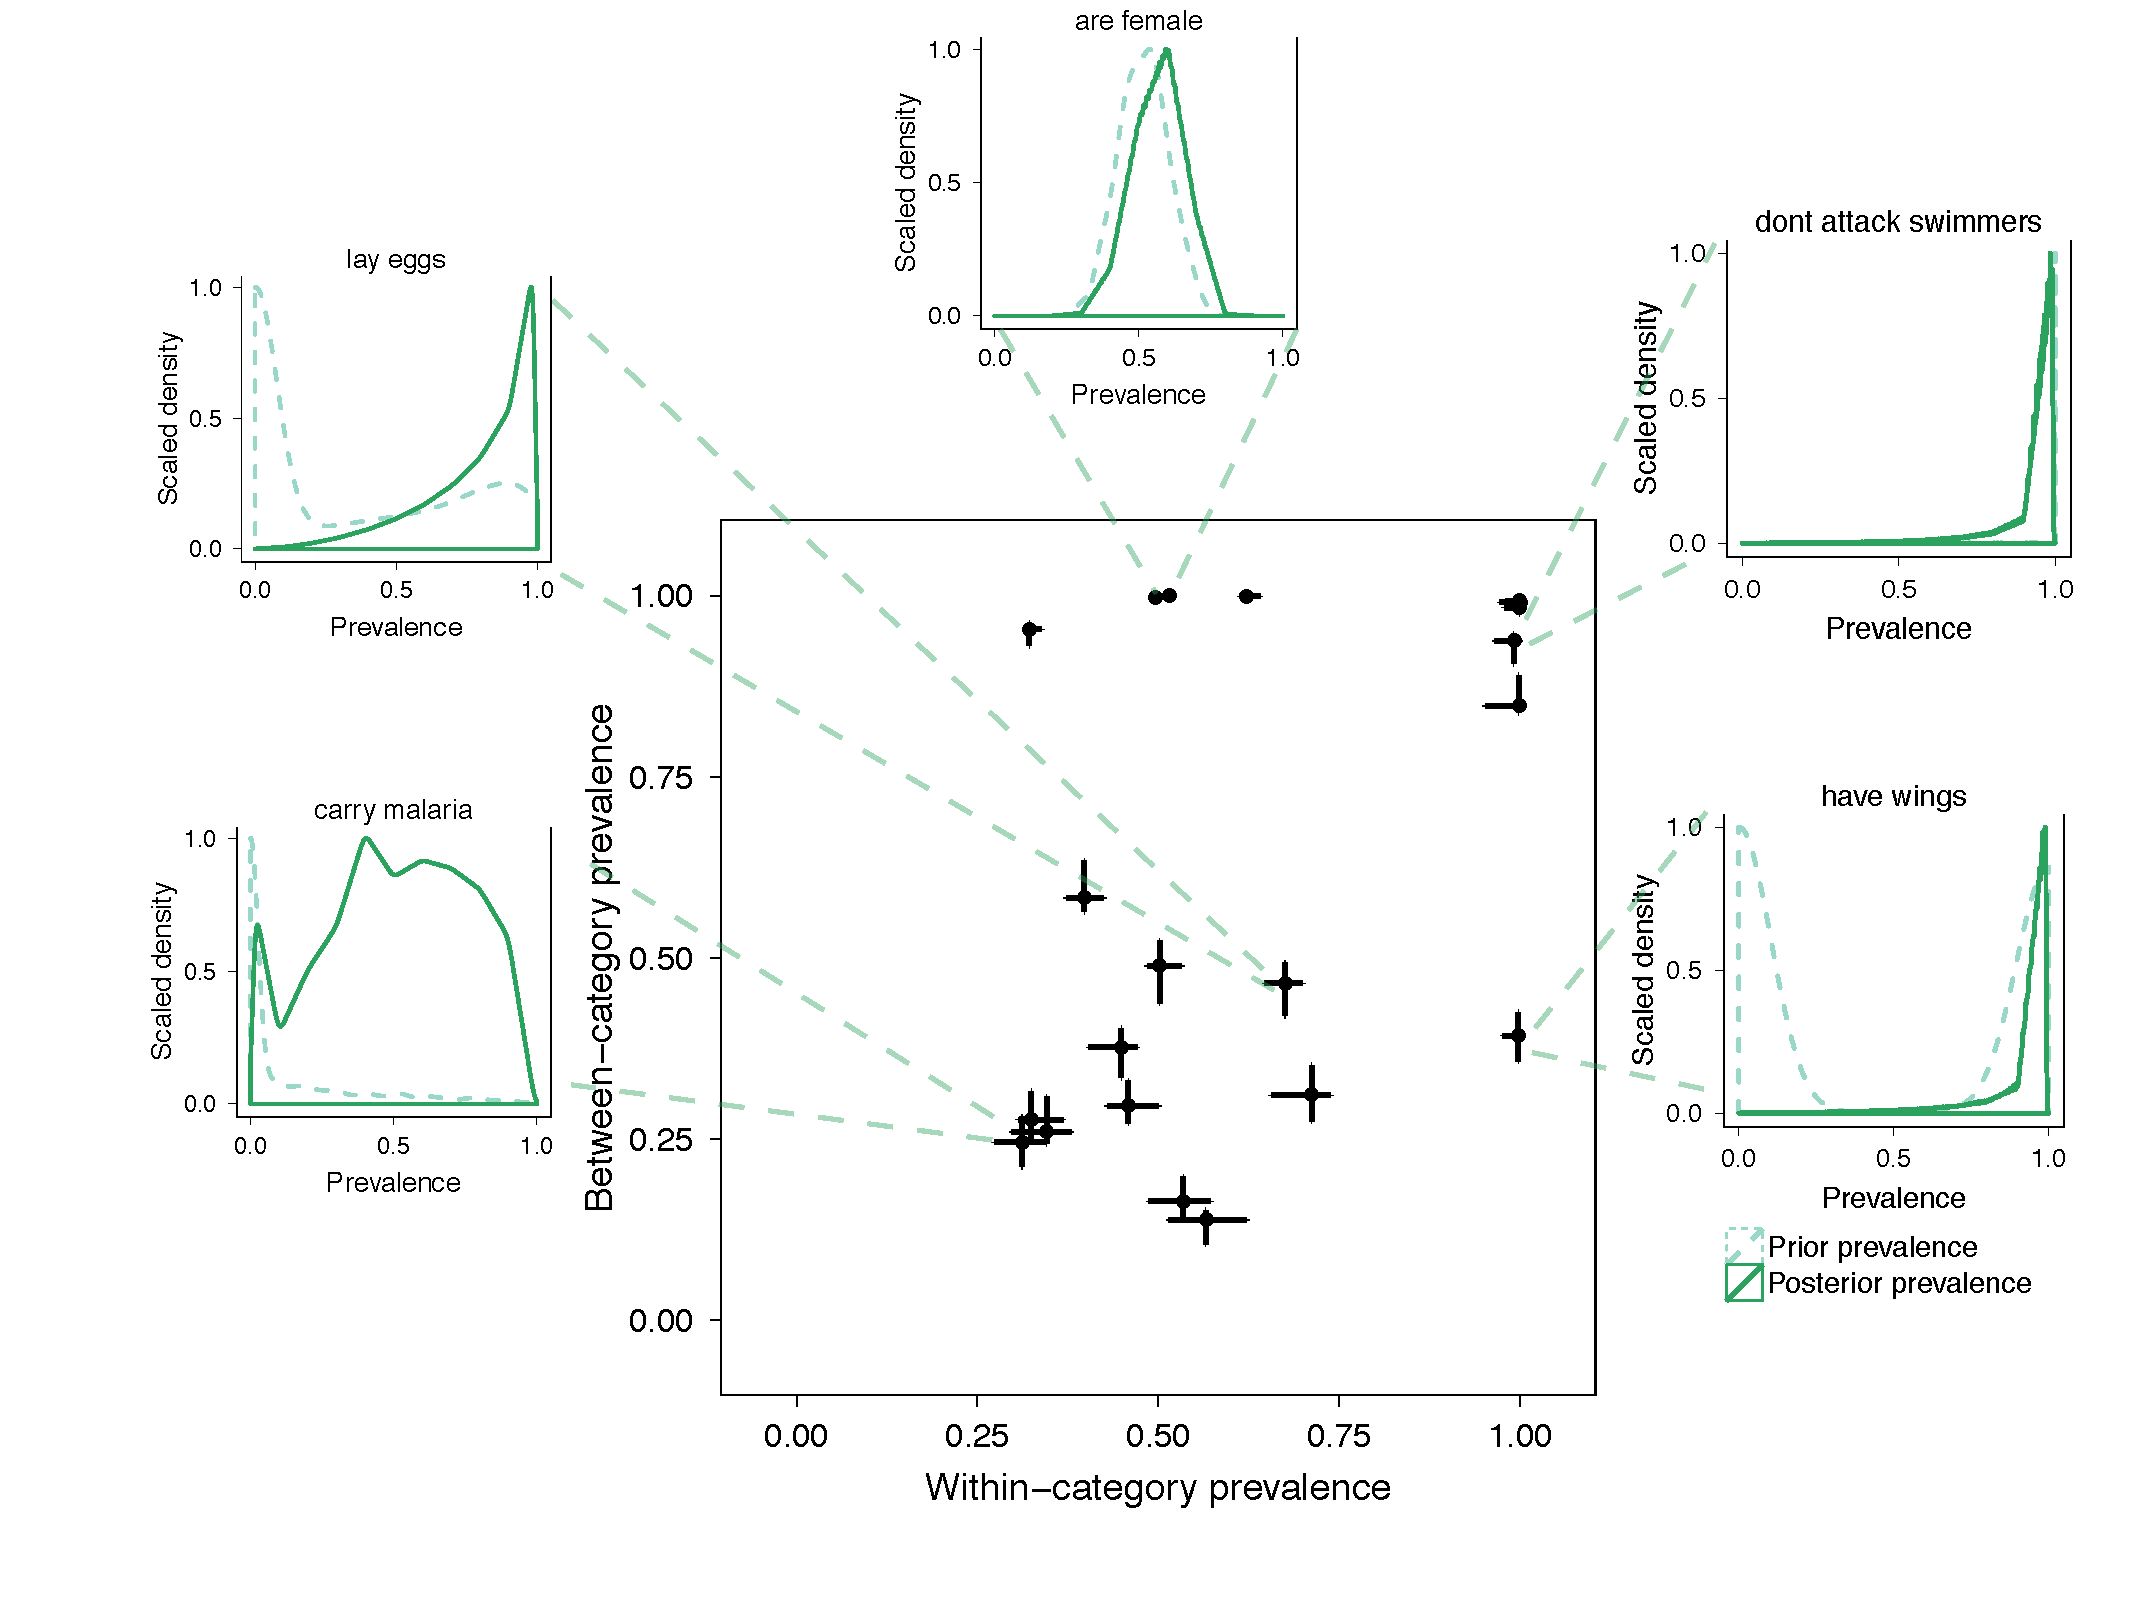
\includegraphics[width=\columnwidth]{prevalence-scatter-wDists.pdf}
    \caption{Prevalence prior distributions empirically elicited for twenty-one animal properties.
    Prior distributions are summarized by the property distinctiveness (relative density at 0\%) and the mean prevalence conditional on the property being present in the kind (mean of density excluding 0\%).
    Pop-out plots display example empirical prior distributions over prevalence together with corresponding model predictions: the posterior after hearing a generic utterance. 
    Intervals on the top of plots show human beliefs about the prevalence of the property within the target category.
%    Posterior distributions show what happens to a listener's belief about the prevalence after hearing the associated generic. 
    Felicitous generic utterances result when the target prevalence is more likely under the posterior than under the prior.
 %   \ndg{should mark the observed within-category prevalence for target kinds in pop-outs? or maybe one of the axes of main plot should be that?}
    }
  \label{fig:priors1a}
\end{figure}

Do subjective beliefs about the prevalence of properties within kinds predict the felicity of generic utterances?
From the prevalence-prior data, we can also estimate participants' beliefs about the prevalence of a property for a given kind (e.g. the percentage of birds that lay eggs; see Supplement (Table 2) for Maximum A-Posteriori (MAP) estimates and 95\% Bayesian Highest Density Intervals (HDI) over the mean prevalence for each property--category pairing). %We first compare the predictions of Eq.~\ref{eq:S2} to 
As a simple baseline hypothesis, we first explore whether these prevalence values themselves predict generic endorsement (e.g.~does the fraction of \textsc{robins} that \textsc{lay eggs} predict the felicity of \emph{Robins lay eggs}?).
A little over half of the variance in truth judgments data is explained by the prevalence of the property within the category alone ($r^2 = 0.599$; Supplement Figure 1). 
This is, of course, expected given the usage of high-prevalence true generics (e.g. ``Leopards have spots.'') and low-prevalence false generics (e.g. ``Leopards have wings.''). 
However, large deviations from a purely target-category prevalence account remain: Generics in which the target category had intermediate prevalence (prevalence quartiles 2 and 3: $ 20\% < prevalence < 64\%$), were not explained at all by prevalence within those categories ($r_{Q2,3}^2 = 0.029$).

\begin{figure}
\centering
    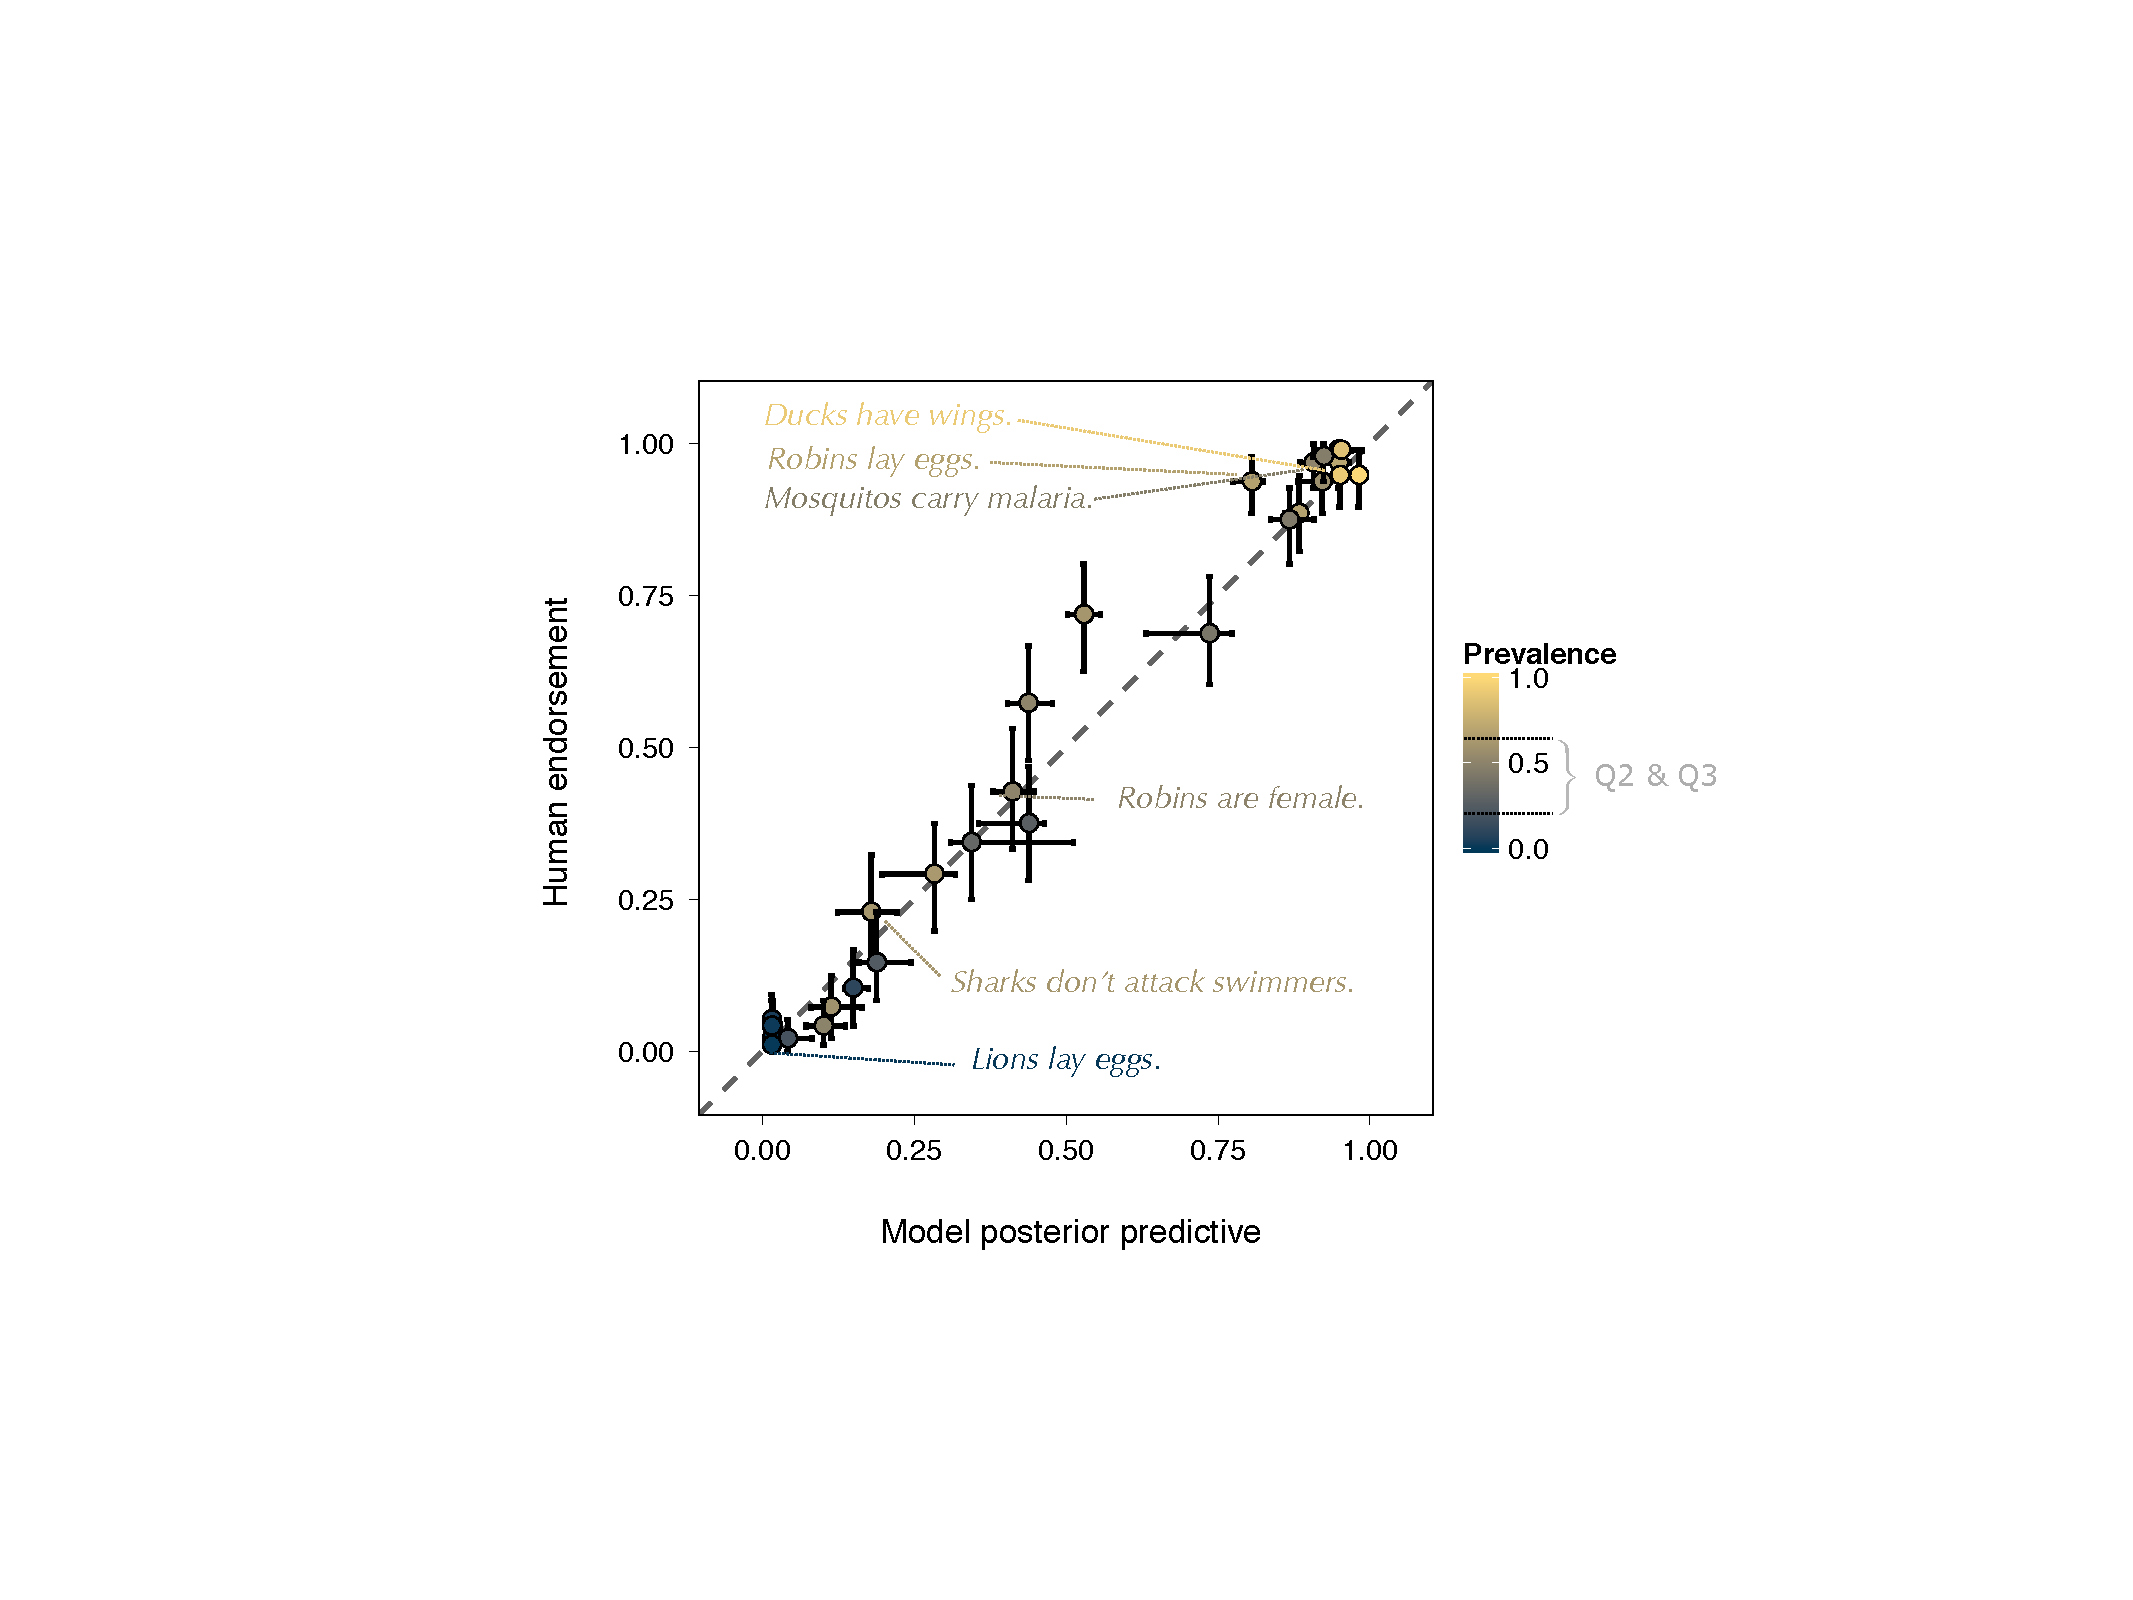
\includegraphics[width=0.7\columnwidth]{truthjudge-scatter-wLabels.pdf}
    \caption{Human acceptability judgments and model predictions for thirty generic utterances about familiar animals and properties. 
    Color denotes target-category prevalence of the property, with darker colors indicating lower prevalence. 
    Error bars correspond with 95\% bootstrapped confidence intervals for the participant data and 95\% highest probability intervals for the model predictions.
    }
  \label{fig:modeldataBars}
\end{figure}

%\begin{figure}
%\centering
%    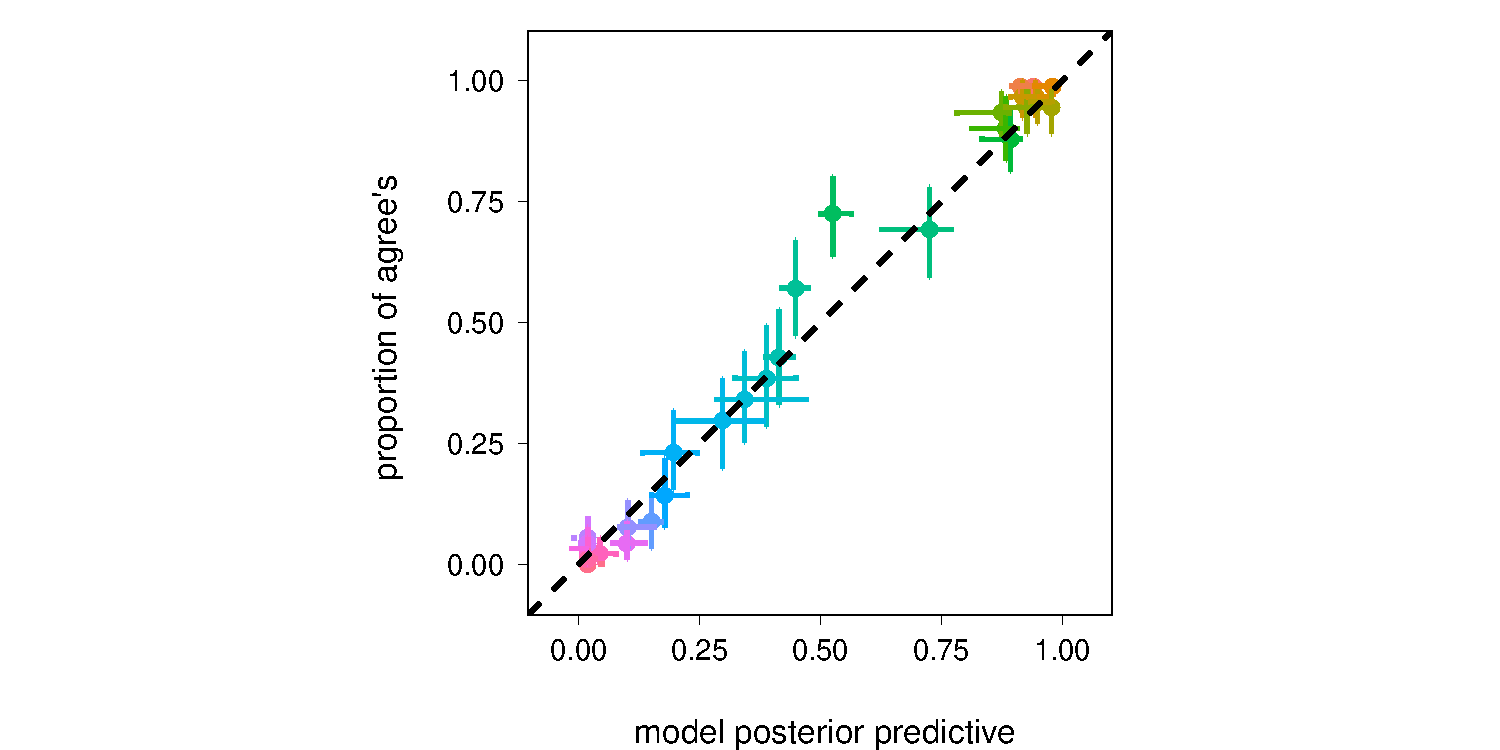
\includegraphics[width=\columnwidth]{tj_n100_tjVsPostpred_95hdi.pdf}
%    \caption{Truth judgments from Expt.~1b for each item vs. the posterior predictive MAP estimates for the target item using the lifted-threshold model with the empirical priors elicited in Expt.~1a. Color spectrum corresponds to the rank ordering of the truth judgment data; similarly colored dots received similar truth judgments. Error bars correspond with 95\% bootstrapped confidence intervals for the participant data and 95\% highest probability intervals for the model predictions.}
%  \label{fig:modeldataScatter}
%\end{figure}

The probabilisitic pragmatics model, using empirically measured priors, does a much better job of explaining the truth judgments ($r^2=0.981$; Figure \ref{fig:modeldataBars}, Supplement Figure 4). 
Generics that received definitive agreement or disagreement are predicted to be judged as such by the model (corners of Figure \ref{fig:modeldataBars}), including items for which target-category prevalence is not a good indicator of the acceptability (for prevalence quartiles 2 and 3, $r_{Q2,3}^2=0.955$; Figure \ref{fig:modeldataBars} lighter shades in the lower left, darker shades in the upper right). 
The probabilistic pragmatics model accounts well for the puzzling flexibility of generic truth-conditions.

\subsubsection*{Generics have strong implications (2300 words to this point)} 

%Generic language exhibits mysterious behavior not only in when it is truthfull but in how it is understood.
Generics ``once accepted [...] appear to be commonly taken in a rather strong sense, as if the qualifier \emph{always} had implicitly crept into their interpretation'' (\citeA{Abelson1966}, Cf.~\citeA{Cimpian2010}). %\red{[Note: this is the same quote that Cimpian2010 use... is this okay?}.
%\mht{Another sentence about why the interpretations are important? / discussing Abelson's quote}
%
Consistent with these musings,
\citeA{Gelman2002} found that adults interpret novel generic statements about familiar kinds (e.g. ``Bears like to eat ants.'') as implying that almost all of the category have the property (e.g. almost all bears like to eat ants).
%\citeA{Cimpian2010} found similar inferences with generics about unfamiliar kinds (e.g. ``Lorches have purple feathers.''). 
How does generic language get interpreted so strongly if the criterion for endorsement is so flexible? 


Interpretations of generic language are readily explored in our model of a listener (Eq.~\ref{eq:L1}) who hears a generic and is trying to infer how widespread the property is. 
We test experimentally how beliefs are updated by generic language using novel animal categories (e.g. \textsc{lorches}), following 
\citeA{Cimpian2010}.
%by using novel animal categories and properties (e.g. \emph{Lorches} and \emph{have green feathers}) to explore how generic language updates one's beliefs. 
%It is strange to measure participants' beliefs about these novel category---property pairs directly (e.g. answering ``How many lorches have purple feathers?'', without knowing what a lorch is).
%Instead, we took advantage of the latent structure in the prior elicitation task (Expt.~1a) to ask participants ($n=40$) about the prevalence of a property (e.g. ``has purple feathers'') across-categories (e.g. ``How likely is it that \emph{there is a} lorch that has purple feathers?'') and within-categories (e.g. ``Suppose there is a lorch with purple feathers. What percentage of lorches do you think have purple feathers?''), separately. 
%We used a hierarchical Bayesian approach to reconstruct the prevalence priors of a similar form to Expt.~1a (see Section \ref{sec:bda2} for details).
Beliefs about the prevalence of properties differ by type of property, including relatively fine distinctions between properties that are all biological in nature \cite{Nisbett1983}. 
We used 5 different types of properties to explore a range of prior beliefs about prevalence: biological parts (e.g. \textsc{have claws}), color adjectives about parts (e.g. \textsc{have green feathers}), vague adjectives about parts (e.g. \textsc{have small wings}), and common accidental or disease states (e.g. \textsc{have wet fur}) and rare accidental or disease states (e.g.  \textsc{have broken legs}) \footnote{The distinction between common and rare accidental properties was determined empirically by analyzing the data first by item, and performing a median split based on the \emph{a priori} mean within-kind prevalence of the property.}.


\begin{figure}
\centering
    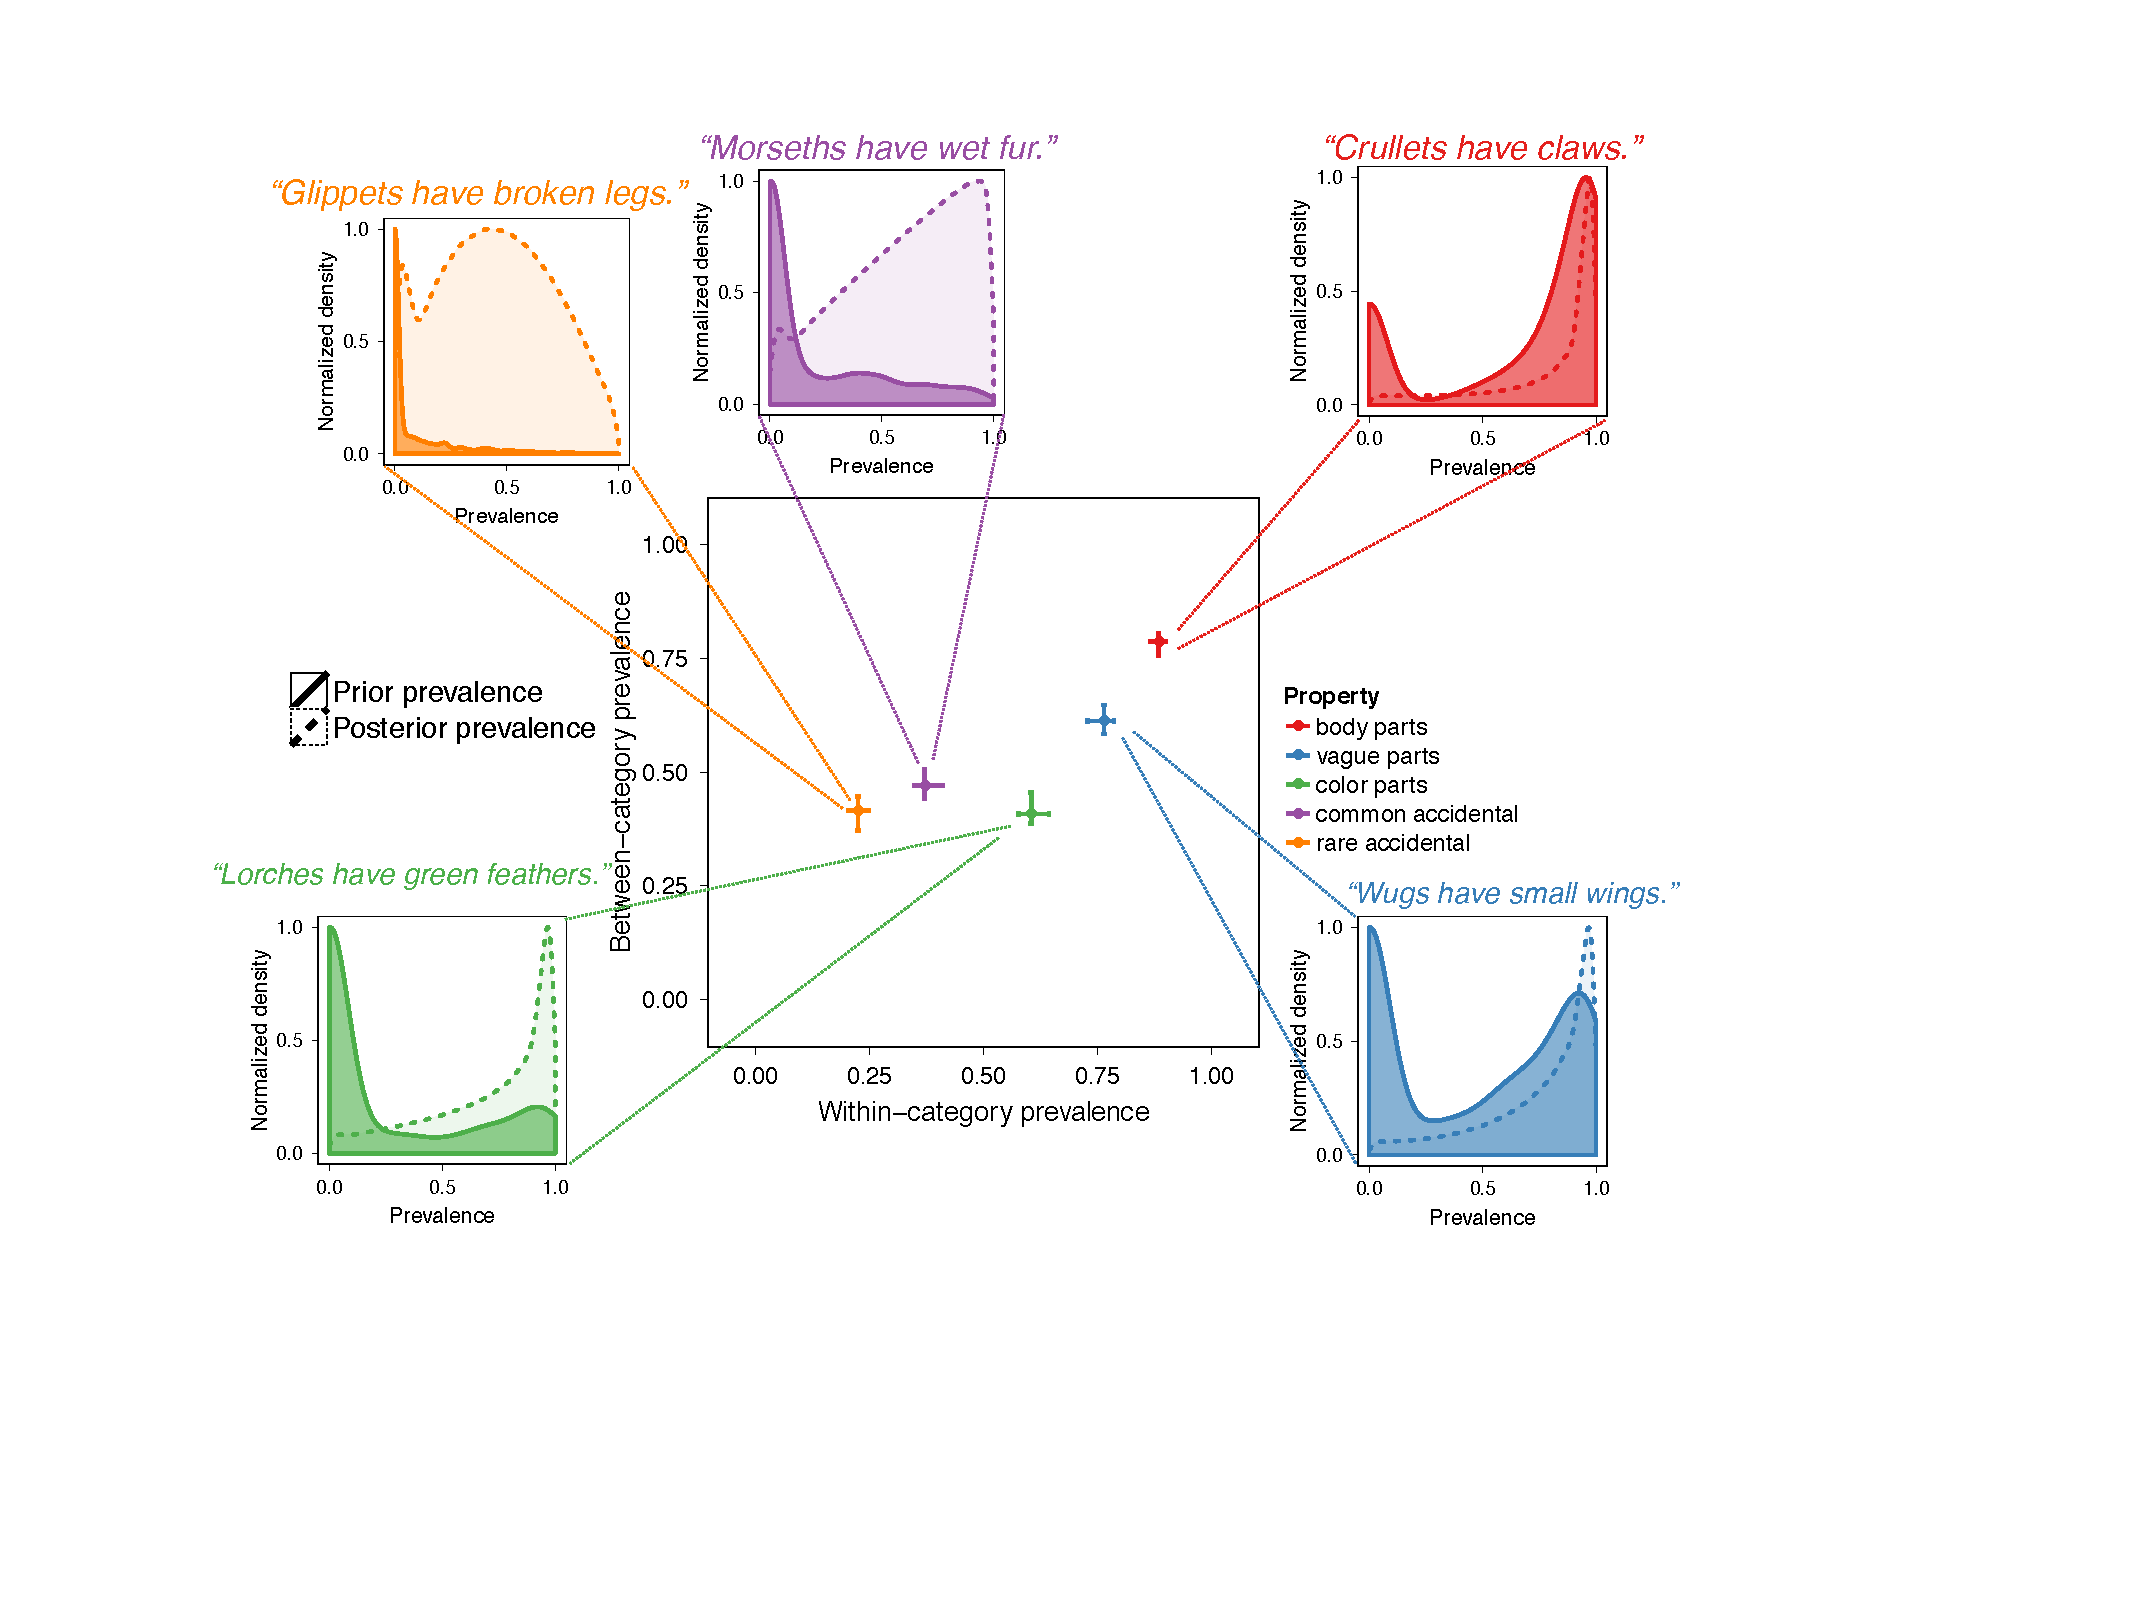
\includegraphics[width=1\columnwidth]{prevalence-asymmetry-scatterwDists.pdf}
    \caption{Prevalence priors for five types of animal properties, plotted on a two-dimensional between- and within-category prevalence space. 
    Pop-out plots show full prior distributions over prevalence and posterior distributions after hearing a generic that corresponds to that type of property. }
  \label{fig:prior2}
\end{figure}

The pragmatic listener in Eq.~\ref{eq:L1} is sensitive to the type of property (and its corresponding distribution on prevalence $P(x)$) when it hears a novel generic.
Particularly, the \emph{a priori} mean within-kind prevalence will guide interpretation as it describes the distribution assuming the property is present.
Again, $P(x)$ was measured empirically ($n=40$, see Supplement Section C).
The five property types fell on a continuum of \emph{a priori} mean conditional prevalence (Figure \ref{fig:prior2}; x-axis). 
Biological properties are expected \emph{a piori} to be more prevalent within a kind than accidental properties, with fine-grained differences even among types of biological and accidental properties.
For instance, within a given kind, colored body parts (e.g. \textsc{green wings}) are expected \emph{a priori} to be less prevalent than some gradable adjectives (e.g. \textsc{small wings}). 
Some accidental properties are expected to be relatively more prevalent \emph{a priori} than others (``common accidental'' vs. ``rare accidental''; e.g. \textsc{wet fur} vs. \textsc{broken legs}; Figure \ref{fig:prior2}, orange and purple plots).
The shapes of the distributions are importantly different as well (Figure \ref{fig:prior2} density plots). 
%Figure \ref{fig:prior2} shows the distinctiveness and mean within-kind prevalence ratings for the empirically measured prior distributions of prevalence $x$ for the 5 different types of properties. 
%Also shown are the computational model predictions for the resulting posterior distributions.
Biological properties (``biological parts'', ``vague parts'', ``color parts'') are bimodal with peaks at 0\% and near-100\% prevalence. 
This distribution updates to a concave posterior distribution peaked at 100\% after necessarily ruling out the 0\% possibility upon hearing \emph{Ks have F} (Figure \ref{fig:prior2}; red, blue and green plots). 
Accidental properties (``rare'' and ``common'') follow unimodal prior distributions and update to convex posterior distributions, reflecting a higher degree of residual uncertainty after hearing the generic utterance as compared to the biological properties. 

%These distributions are not necessarily peaked at 100\%, and the expected 
%Figure \ref{fig:prior2} (right) shows the region of interest of these distributions by removing the mass at 0. %
%With the exception of the body part category, properties are mostly likely to be absent from the category (Figure \ref{fig:prior2} left; modes of distributions are at 0).
%If the property is present in the category, the most likely prevalence for biological properties (``part'', ``color part'', and ``vague part'') is 100\% (Figure \ref{fig:prior2} right; modes of blue, green, and red distributions are at 1).
%This is not the case with the prevalence priors for accidental properties, for which lower values are more likely (Figure \ref{fig:prior2} right; modes of orange and purples distributions are at some low prevalence).



We compared the interpretations of the pragmatic listener in Eq.~\ref{eq:L1} to human judgments ($n=40$) about the likely prevalence of the property after hearing a generic (e.g. \emph{Lorches have green feathers.}), in the same spirit as \citeA{Gelman2002}. 
Also following \citeA{Cimpian2010}, we recruited participants ($n=40$) to help determine the average prevalence at which a speaker would assent to the generic, which was previously found to be not as sensitive to participants beliefs about the property (but, cf. \citeA{Cimpian2010}, Expt.~4).
We used the speaker model (Eq.~\ref{eq:S2}) again to predict this truth judgment task (as we did previously for the naturalistic generics).
We submitted our speaker model to the same analysis as the truth judgments data, following \citeA{Cimpian2010} (see Supplement Section D). 

Human prevalence judgments after reading the generic were affected by the type of property in question and its corresponding mean conditional prevalence (Figure \ref{fig:exp2b} Left; solid line): The more prevalent a property is expected to be \emph{a priori}, the stronger the implications of a generic ($\beta = 0.59; SE = 0.08; t(39) = 7.14; p < 0.001$)\footnote{These statistics are the result of a mixed-effects linear regression with a maximal mixed-effect structure: Random by-participant effects of intercept and slope}. 
However, the generic does more than merely inform a listener that the property is present: 
A generic carries the communicative force of a speech act, and thus implies the property is \emph{more prevalent} than a listener would expect (Figure \ref{fig:exp2b} solid line lies above $y=x$ line).
The listener model (Eq.~\ref{eq:L1}) produced the same strong interpretation along a gradient (Figure \ref{fig:exp2b}, Right, solid line), displaying the sensitivity to abstract beliefs about the properties that human participants show. 
The speaker model did not make appreciably different predictions as to the average prevalence to accept the generic, consistent with the intuition that generics are acceptable for a wide range of prevalence levels; a similar absence of a gradient was observed in the human data ($\beta = 2.82; SE = 4.02; t(39) = 0.70; p = 0.49$; Figure \ref{fig:exp2b}, dotted lines). 
The listener and speaker pair of models predicts human endorsements and interpretations of novel generic utterances well ($r^2(10) = 0.921$)\footnote{We performed a by-item analysis for the implied prevalence data and found a similar strong fit to the data ($r^2(40) = XXX$; see Supplement Section D5)}. 

%Interestingly, we observe greater implied prevalence of common accidental properties than rare accidental properties, given our median split based on the prior elicitation task ($\beta=0.061; SE = 0.025; t(39) = 2.47; p = 0.018$) \footnote{These statistics are the result of a mixed-effects linear regression with a maximal mixed-effect structure: Random by-participant effects of intercept and slope}.
%Implications of generics of body parts was significantly greater than those of the biological properties used by \citeA{Cimpian2010} (here, ``color parts'') ($\beta=0.118; SE = 0.024; t(39) = 4.74; p < 0.001$).
%There was also a trending effect for the implications of vague body parts (e.g. curly fur) to be greater than those of color parts (e.g. yellow fur) ($\beta=0.032; SE = 0.016, t(54.8) = 1.95; p = 0.056$), possibly due to the belief that the same kind of animal can come in many different colors (e.g. dogs).

\begin{figure}
\centering
    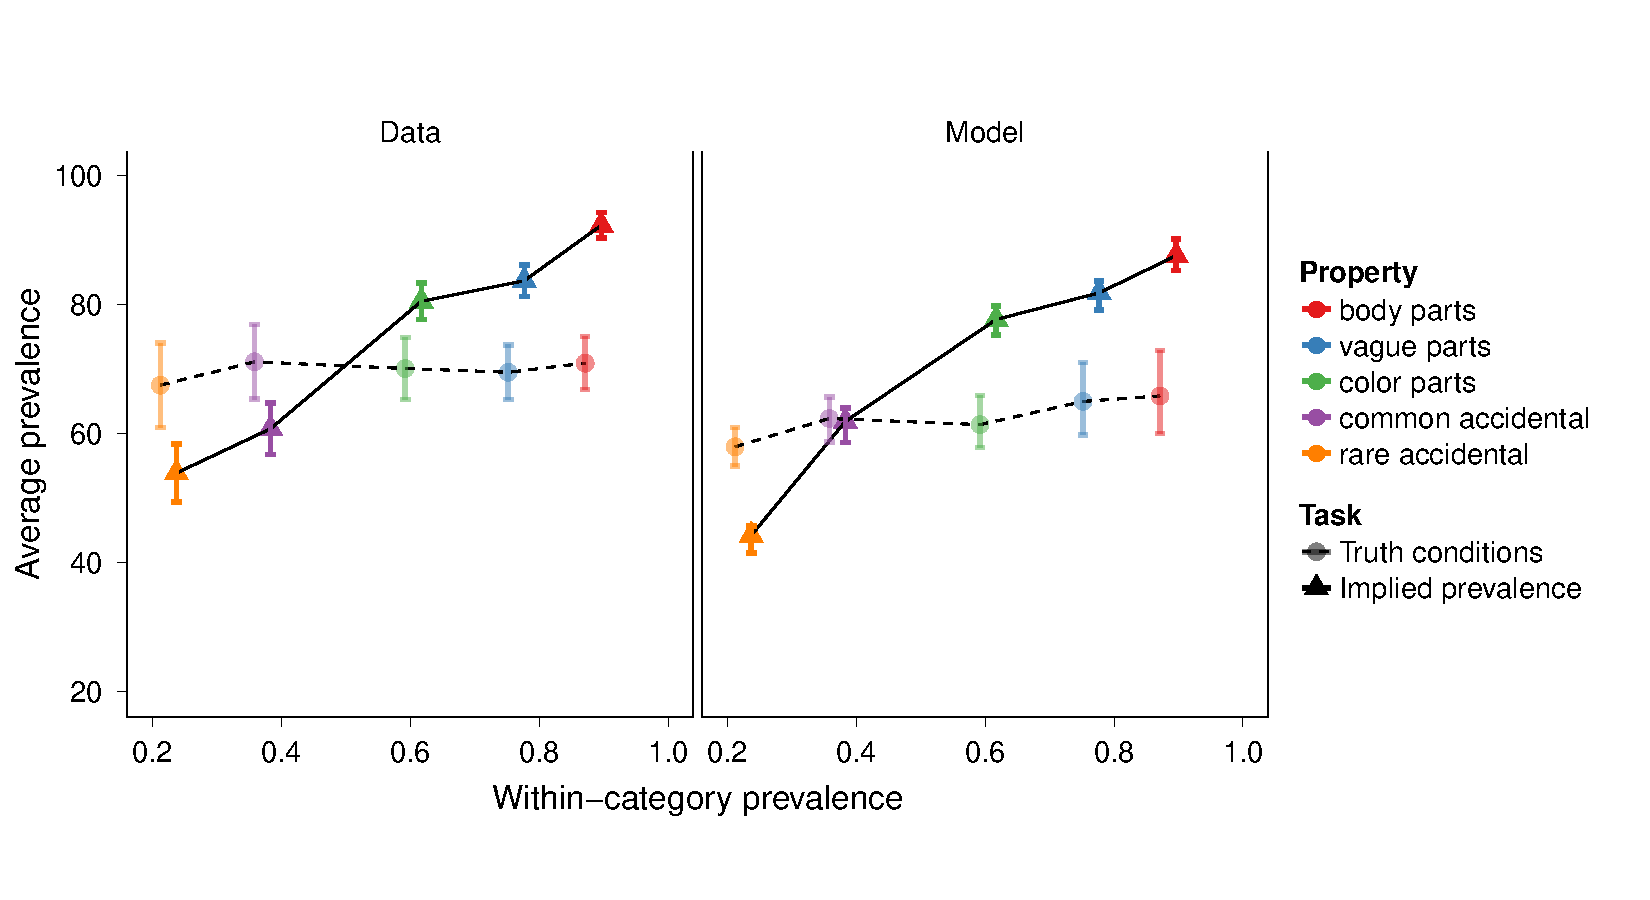
\includegraphics[width=1\columnwidth]{asym-lines-data-model-2phi-2so-50kx3.pdf}
    \caption{Human judgments and model predictions of prevalence implied by novel generic utterances (implied prevalence task; solid line) and average prevalence that leads to an acceptable generic utterance (truth conditions task; dotted line) as it relates to the \emph{a priori} average within-category prevalence.
    $y = x$ line denotes the prevalence inferred upon knowing the property is present in the kind. 
    For each kind of property, the generic utterance implies a higher than expected prevalence.
    Generic statements about biological properties, imply that high proportion of the category has the property, for both human participants and the model (solid line: red, blue and green). 
    Generics about accidental properties do not result in such a high implied prevalence (solid line: purple and orange).  
	While the implications of generic utterances are highly variable across the different types of properties, the average prevalence that leads to an acceptable generic does not vary, for participants or the model.
        %Generic statements are accepted for a range of prevalences, resulting in a intermediate average prevalence (dotted line) that deoesn't vary by property type for the truth conditions task. 
    Error bars denote bootstrapped 95\% confidence intervals for the data and Bayesian 95\% credible intervals for the model.
%    \ndg{change x-axis label to "a priori expected prevalence" or something like that -- "within-category prevalence" is ambiguous.}
}
  \label{fig:exp2b}
\end{figure}


%Consistent with the effects reported by \citeA{Cimpian2010}, biological properties (body, vague, and color parts) have stronger interpretations than their truth conditions would suggest (Figure \ref{fig:exp2b}; solid vs. dotted lines; green, blue and red points), whereas accidental properties receive more modest interpretations (orange and purple points).



%How does the model capture these fine-grained inferences that listeners draw?
%Consider again the belief distributions about the properties inferred from Expt.~2a (Figure \ref{fig:prior2}). 
%All of the properties have substantial mass at 0 (Figure \ref{fig:prior2} Left). 
%This gives the speaker validity in saying the generic at low prevalence levels (though the speaker's confidence in doing so increases as prevalence increases).
%The listener has the complementary task: She brings \emph{a priori} uncertainty about the generic threshold to the table.
%Consider what would happen if she inferred the most conservative threshold (0) and responded with the \emph{maximum a posteriori} (MAP) of the distribution. 
%A threshold of 0 produces Figure \ref{fig:prior2} (right), because it only rules out the possibility that 0\% of the category has the property. 
%The resulting peaks (MAPs) of the distributions are near 1 for biological properties (parts, color parts, vague parts) and around 10\% for accidental properties (both rare and common). This alone would produce variable interpretations. 
%Our listener, however, does something wiser: She integrates over her uncertainty about the threshold (believing the speaker to be not just truthful but informative as well), and produces interpretations that both take reflect the whole distribution.
%This results in subtle differences between the implications of body parts (e.g. ``Lorches have wings.'') and  color parts (e.g.``Lorches have purple wings.''), and differences in interpretations of rare and common accidental properties. 
%

\subsubsection*{Conclusions (3200 words up to now)}


We evaluated an explanation of generic language derived from general principles of pragmatic language understanding and a simple but uncertain basic meaning---a threshold on property prevalence.
Our formal model is a minimal extension of the RSA theory of language understanding, together with an underspecified threshold semantics.
The model was able to explain two qualitative puzzles of generics, their extremely flexible truth conditions and the contrastingly strong interpretation of novel generics; it also predicted the quantitative details of participants' judgments with high accuracy.

%generics have a simple but uncertain basic meaning---a threshold on property prevalence---which is refined by social reasoning.
%a minimal extension of a general-purpose probabilistic model of language understanding wherein social-cognitive mechanisms act on uncertainty in the meaning of a generic utterance to produce a less uncertain meaning.
%Model predictions for interpretation of generic sentences depend on the listener's beliefs about the property in question and the communicative force of a speech-act. 
%The model predicted participants' judgements with high quantitative accuracy for both goodness judgements for natural generic sentences, and interpretation of novel generic sentences.
%Our model both the role of the speaker to produce felicitous generic utterances and the role of the listener to interpret those utterances in context, with high quantitative accuracy.
%general-purpose language understanding mechanisms are 



%%this paragraph isn't needed and is confusing....
%Interpretation of generic language is strongly governed by listeners' beliefs about the domain in question. 
%The generic, it would seem, doesn't convey any additional information beyond what the liste	ner already knew about the domain.
%This shouldn't surprise us. 
%In much the same way, ``John is tall'' does not actually tell a listener about what \emph{tall} means\footnote{However, ``John is a person'' does tell a listener about what \emph{tall} means in ``John is tall''.}. 
%Rather, the listener is expected to come to the conversation with some beliefs about heights, and knowing that John is a person, be able to infer likely meanings for \emph{tall}.

Previous psychological and philosophical work on generics has looked beyond prevalence and focused on conceptual distinctions and relations \cite{Gelman2005, Prasada2013, Leslie2007, Leslie2008}. 
\citeauthor{Prasada2013} has argued for a distinction between \emph{characteristic} properties (e.g.~\emph{Diapers are absorbent.}) and \emph{statistical} properties (e.g.~\emph{Diapers are white.}).
\citeauthor{Leslie2007} suggests information that is striking (e.g.~\emph{Tigers eat people.}) is useful and thus permitted to be a generic.
\citeauthor{Gelman2005} outlines how generics express qualities that are relatively timeless, enduring, and essential, and that generic language can increase the psychological coherence of a category.
\citeA{GelmanEtAl2004} finds that child-parent conversations contain many more generics about animal kinds than about artifact kinds, possibly owing to the belief that animal kinds are more richly structured than artifact kinds. 
Where in the prevalence-based semantics could such conceptual distinctions come into play?
Beliefs about prevalence are represented as probability distributions; a framework that is useful for representing rich, structured knowledge of the world \cite{Goodmanconcepts}. 
It is plausible that the prevalence distributions focused on in this work are derived from richer conceptual knowledge, including higher-order conceptual knowledge about the nature of different properties and categories \cite{Gelman2005, Keil1992}. 
That is, for the purpose of the semantics of generics, prevalence may be sufficient to capture the range of truth judgments and interpretations. 
How interlocutors arrive at estimates of the prevalence, and what other inferences are licensed in a context, may be the result of a deeper conceptual model of the world. 

It might seem paradoxical that a part of language that is so common in communication and central to learning should be vague. 
Shouldn't speakers and teachers want to express their ideas as clearly as possible?
To the contrary, such underspecification can be efficient, given that context can be used to resolve the uncertainty \cite{Piantadosi2012}.
In our work, context takes the form of a listener and speaker's shared beliefs about the property in question. 
By leveraging this common ground, generics provide a powerful way to communicate and learn generalizations about categories, which could otherwise be difficult or costly to learn through direct evidence.
%This, coupled with standard inferences from conversational pragmatics, allows the listener to arrive at a specific meaning of the otherwise underspecified utterance.
The dark side of this flexibility is the potential for miscommunication or deceit: A speaker might assert a generic utterance that he himself would not accept, conveying a too-strong generalization to a na\"{i}ve listener.  
Our model predicts this potential particularly for properties which, which present, are widespread in a category---we showed that biological properties are believed to have this distribution, but many properties of social categories may as well \cite{Cimpian2011a, Cimpian2012b, Rhodes2012}.
%This listener would then have a belief distribution even further from the truth. 


Categories are inherently unobservable. 
You cannot see the category \textsc{dog}, only some number of instances of it.
Yet we easily talk about these unobservables, conveying hard-won generalizations to each other and down through generations.
The model presented here gives one explanation of how we do so, providing a computational perspective on how category generalizations are conveyed and how beliefs play a central role in understanding language.

%Language provides a way to orient to these unobservables, enabling the sharing of observations about these unobservables with others.
%It is inherently a process of reaching in the dark, riddled with uncertainty. 
%Yet cooperation allows interlocutors to align their uncertainty and ensure knowledge can be conveyed.
%This formalism gives a new, computational perspective on how ideas are conveyed and how beliefs play a central role in understanding language.
%Generics are vague, but predictable and useful.


%


\bibliographystyle{apacite}

\setlength{\bibleftmargin}{.125in}
\setlength{\bibindent}{-\bibleftmargin}

\bibliography{generics}


\end{document}
